\section{Protecting Against UI Input Integrity Manipulation Attacks}
\label{sec:fieldSwap}


\iffalse
In the previous section, we described how \device defends against the attacker's manipulation of input values. In this section, we describe and propose a solution for more sophisticated attacks that compromise the integrity of users' input by manipulating graphical elements on the browser. Our attacker model remains identical to the previous solution, i.e., an attacker that compromises entire host system and the network communications. The malicious host can employ manipulation on the graphical interface elements such as adding extra fields or removing some of the fields. This type of data is effective against inexperienced users who are not properly familiar with the user interface and the specific input fields in a page. Note that when the server serves a specific website, it knows what to expect when the user submits the data into the browser. Therefore, these attacks can be readily detected by the server using the former method due to the discrepancy in the number of input data.  

If the user is experienced with the user interface, a malicious host can orchestrate a more sophisticated attack that swaps the labels of input fields on the served web page. Here, the attacker does not manipulate input values (since these values will be signed by the \device) but instead presents false labels in the web form to the user. The user is then tricked into entering the data into incorrect fields.

The experienced users who are familiar not only with the user interface, but also know which data fields to expect are not susceptible to such kind of attacks. However, a malicious host can always show a notification falsely claiming that the server updated the UI elements due to a version upgrade. This way the malicious host can trick even a very experienced user into putting data into a wrong field. Therefore, we can conclude that even the most experienced users are susceptible to the UI manipulation attack that compromises users' integrity. 

One can argue that serving a manual or displaying the template (as security indicator) of the website in a separate display (may be attached with the \device) can prevent UI manipulation attack. However, several existing pieces of research~\cite{197283,41927} show that in practice users tend to ignore security indicators. Therefore, one of the design goals of \tool was not to rely on any security indicator that increases user's cognitive load. \tool rather asks the user to perform a compulsory but a very simple task that associate her input data with the field label which she is seeing on the host's screen. We argue that the additional task that the user performs is extremely simple in nature and does not change the natural user behavior in any significant way.

\begin{figure}[t]
  \centering
    %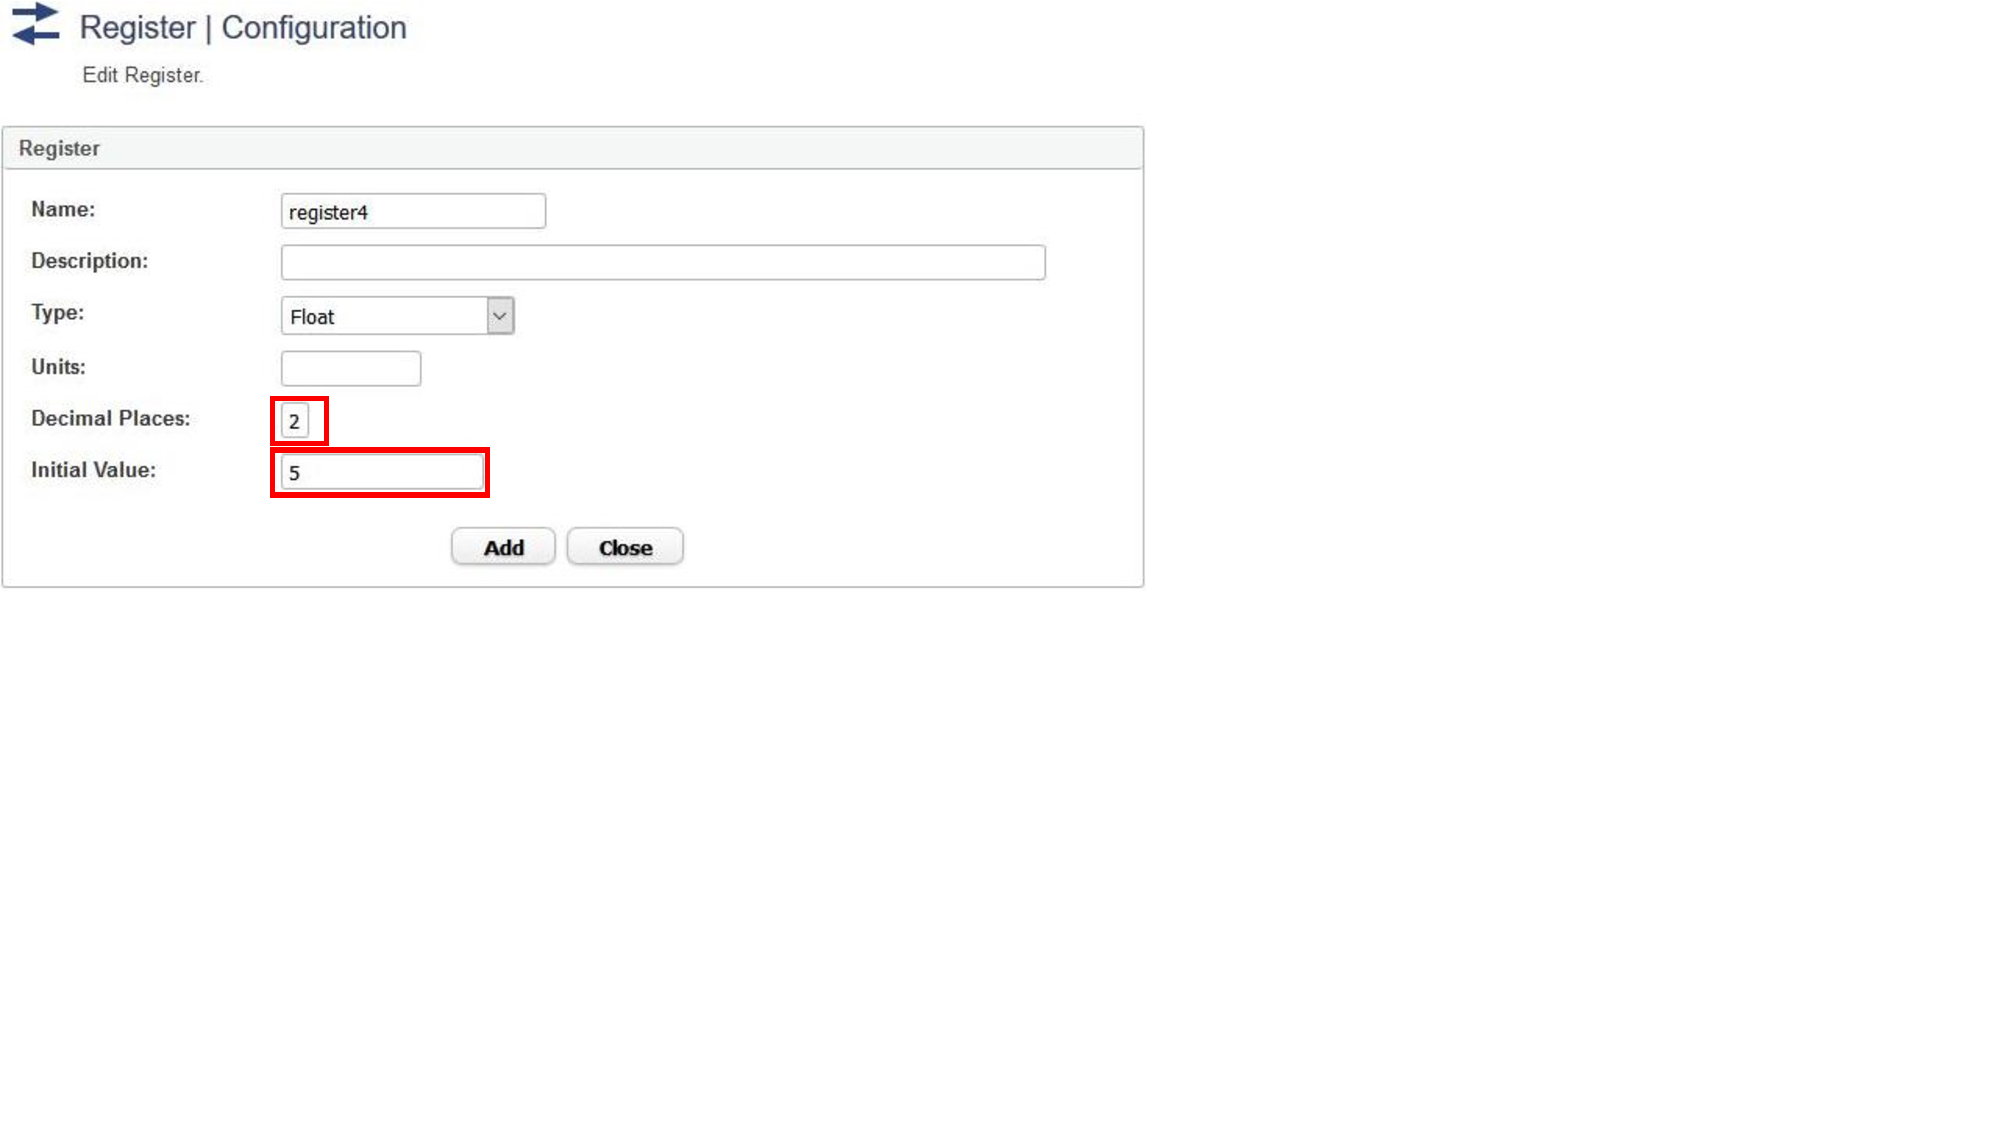
\includegraphics[trim={0 9cm 14cm 0},clip, width=\linewidth]{SwapExample.pdf}
    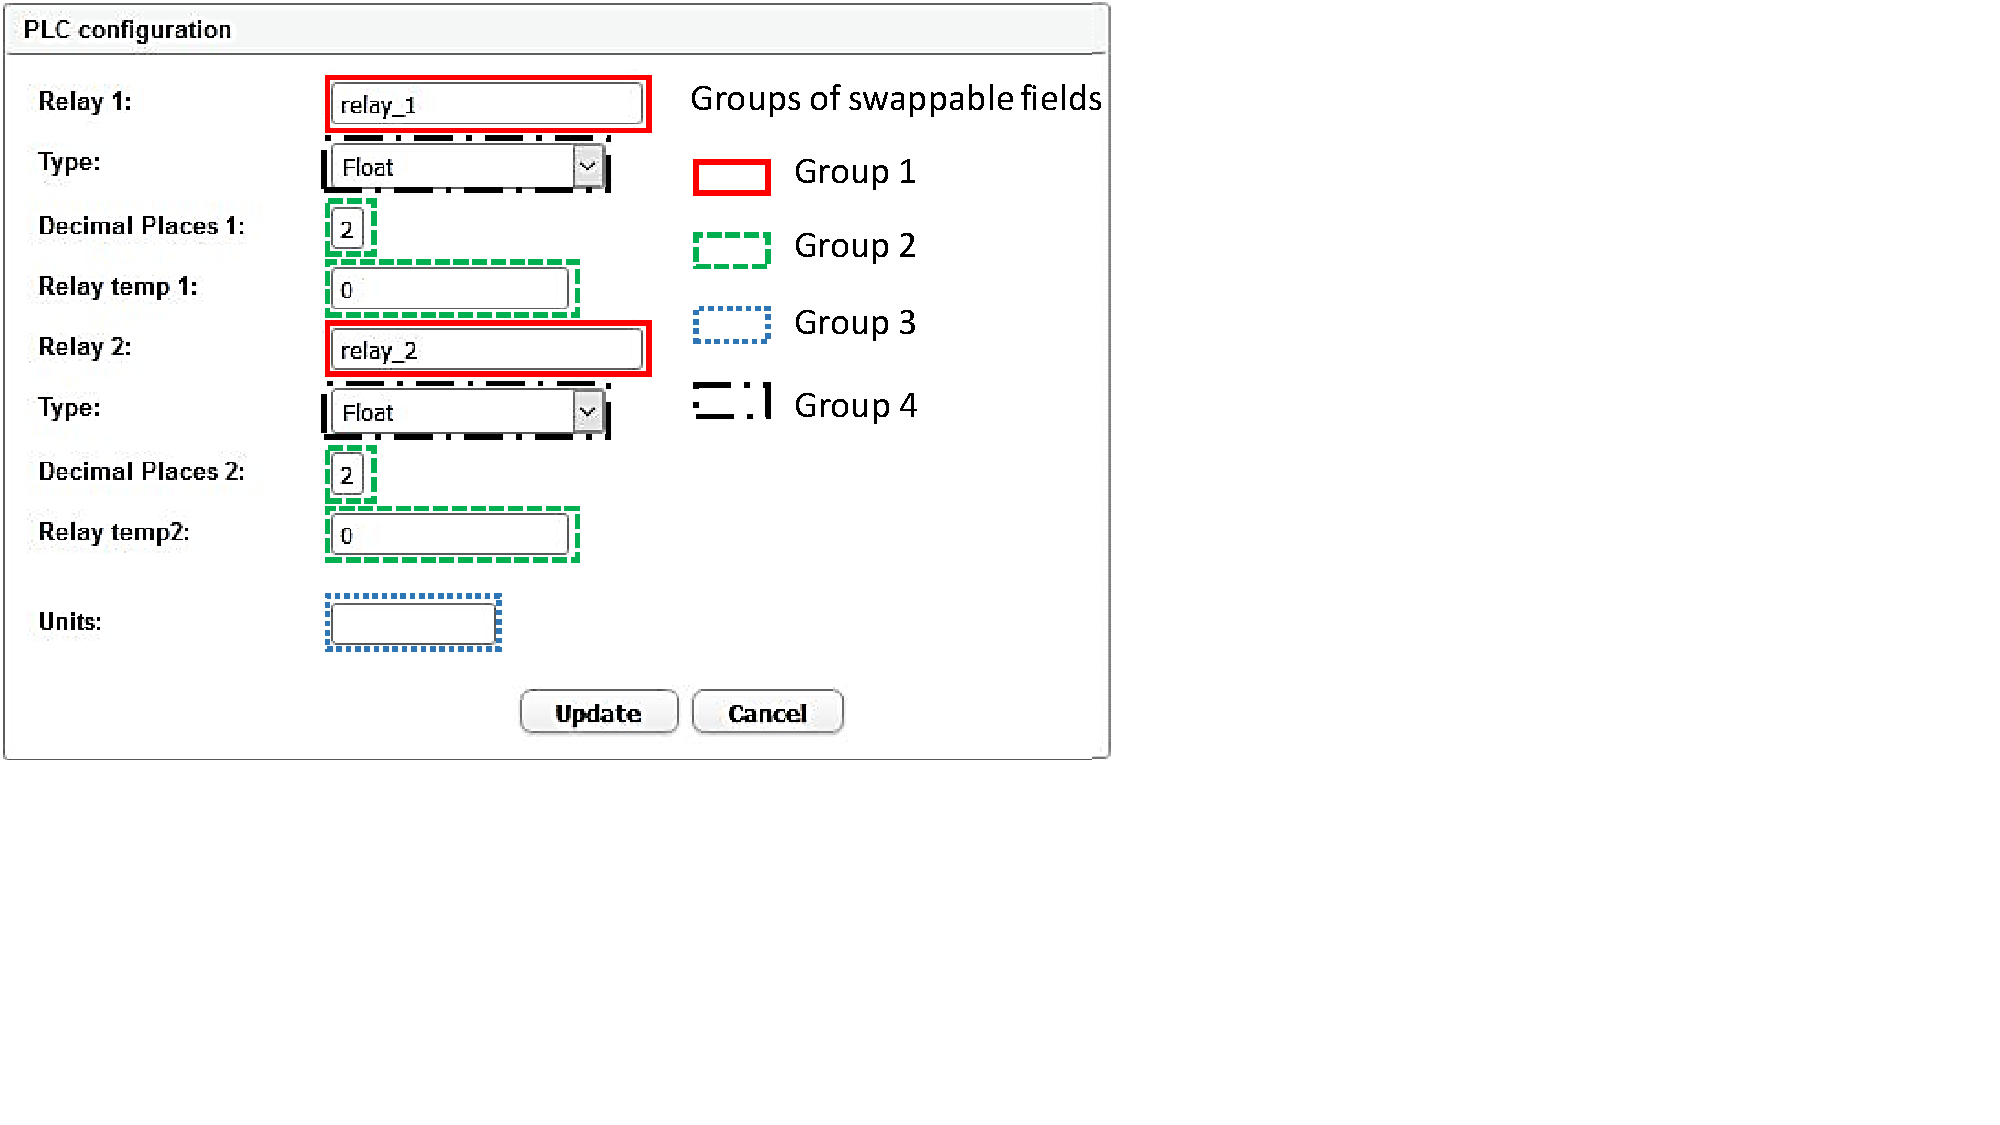
\includegraphics[trim={0 7cm 15cm 0},clip, width=\linewidth]{SwapExample_revised2.pdf}
    \caption{An example of a web-based PLC configuration page where the highlighted fields can be reordered by a malicious host. Note that Relay 1 and Relay 2 are interchangeable, where as Decimal places 1, 2 and Relay temp 1, 2 all are swappable.}
    \label{fig:swapExample} 
\end{figure}


\myparagraph{The attack} Field data types can easily be identical but interchanging the values may change the behavior of the end-system. The \server cannot notice this change since the signed values from the \device will be no different from the values entered through the web form and could be plausible values and entered in a plausible sequence for the served web form. E.g., the attacker can swap the labels of fields 'Decimal Places' and 'Relay temp 1' in the web-form illustrated in Figure~\ref{fig:swapExample}. The user will then enter the values in a sequence ('Relay temp 1', 'Decimal Places'). The server will interpret this as a sequence ('Decimal Places', 'Relay temp 1') since this is the order that should have been imposed by the web form. Since both values are in the expected ranges, the server will not notice the swap, unless these values need to be related (e.g., 'Decimal Places'$<$'Relay temp 1') and the server checks for this relation. However, in many systems, one cannot rely on the end-device logic to check for such consistency and there are many values that will overlap in range but will otherwise be fully independent. Such protections, therefore, do not easily generalize.

\fi

In the previous section, we discuss the technical challenges we faced while designing and developing \tool.  we describe a new attack: UI Input Integrity Manipulation Attack (Section~\ref{sec:systemDesign:challenges:uiAttack}) where the attacker manipulate the user interface elements to trick the users into giving wrong inputs. To prevent this attack, we, therefore, propose a mechanism which binds input data to the input label. There are two parts to this proposed solution, one of which is executed on the server and the other on the \device at the user side.

\subsection{\tool Server Side Tool}
\label{sec:fieldSwap:serverSide}

\begin{figure}[t]
 \centering
 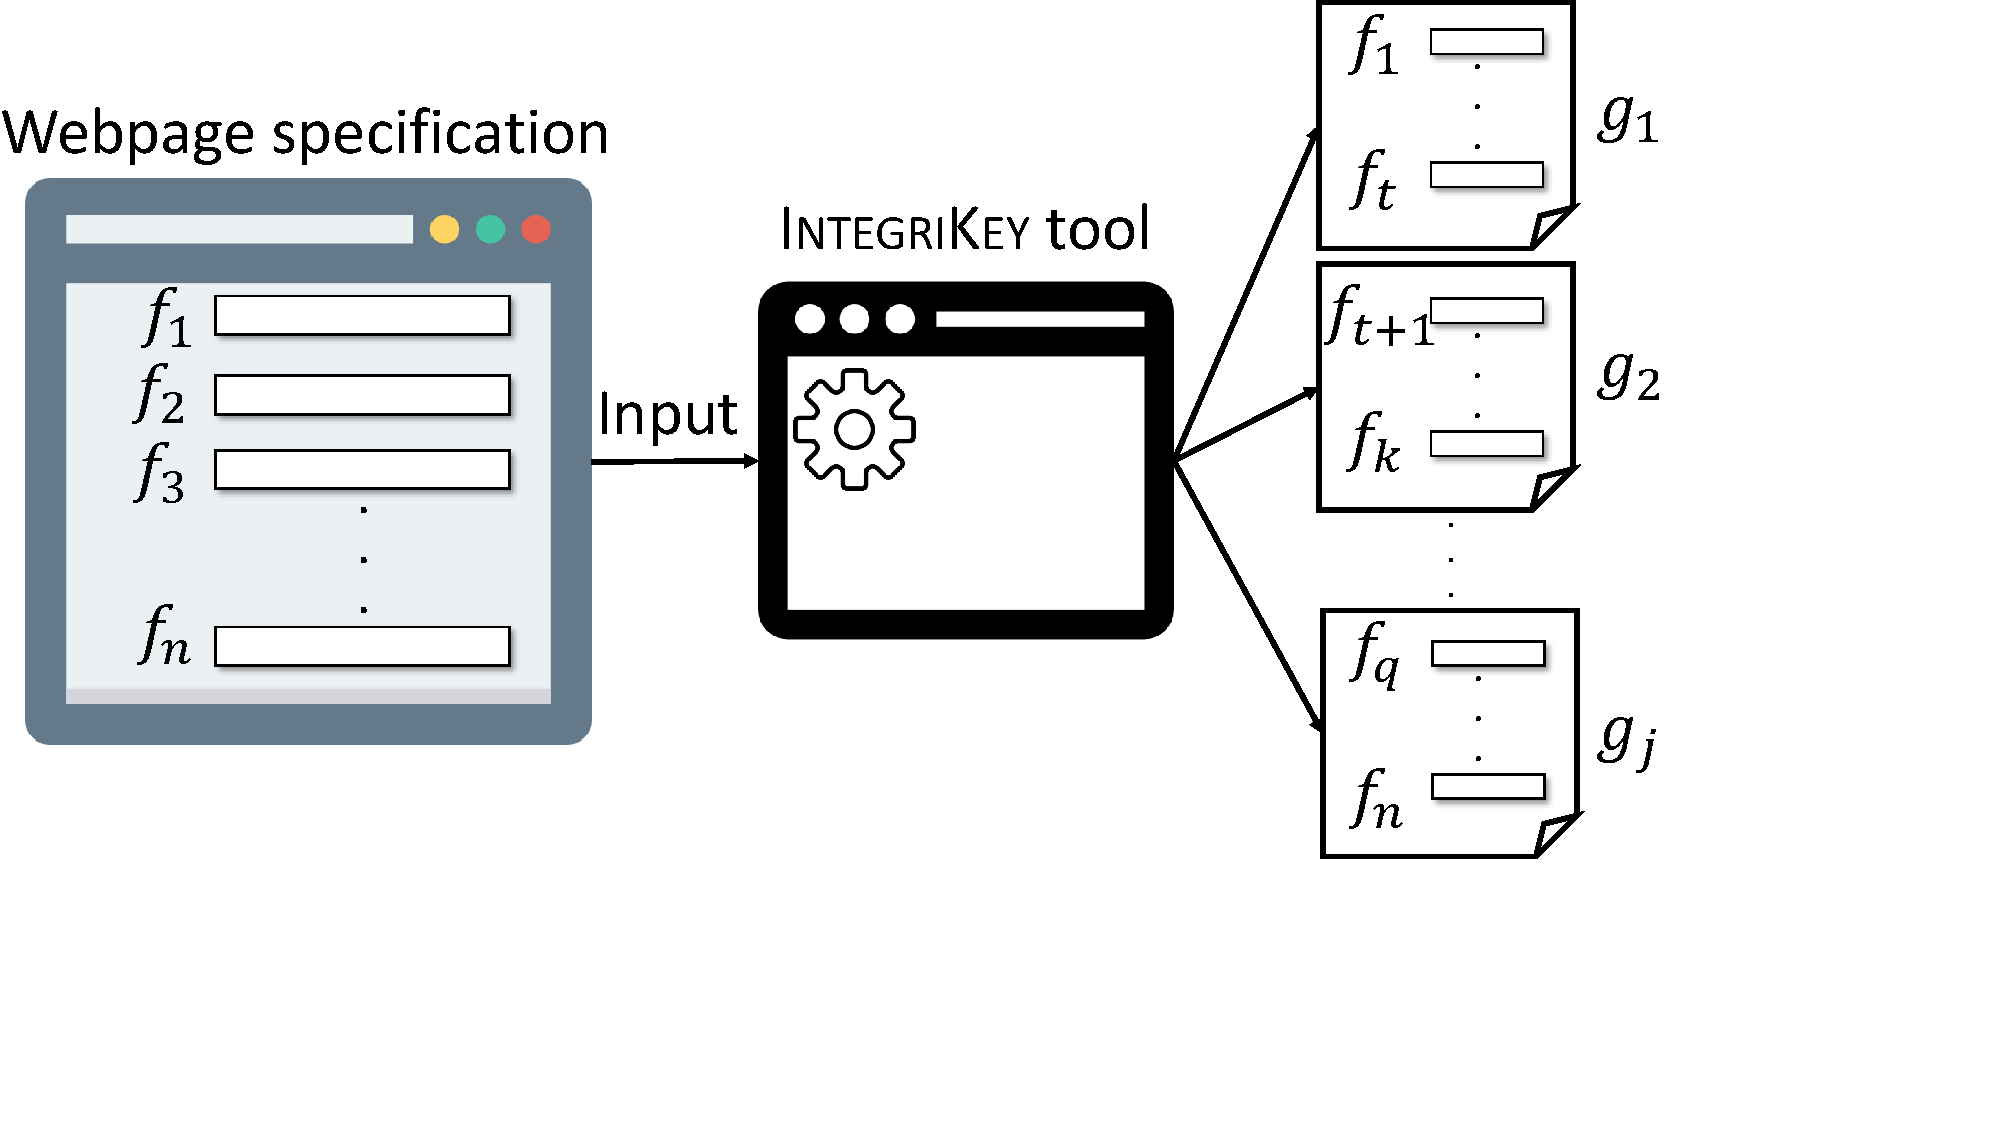
\includegraphics[trim={0 4cm 5cm 0},clip,width=\linewidth]{ServerSideTool_revised.pdf}
% \caption{\bfseries High-level flow of operation of the \name tool at the server side. The tool takes a web page with input fields $f_1, f_2, \ldots, f_n$ and converts it to multiple pages $P_1, P_2, \ldots, P_j$ where each page holds a distinct subset of the original input fields. The pages are configured in a way that no two labels of input fields within a single page and no two pages can be swapped.}
 \caption{High-level flow of operation of the \name tool at the server side. The tool takes a web page specification with $n$ input fields $f_1, f_2,\ldots f_n$ and converts it to set of subsets of the original fields $g_1, g_2, \ldots, g_j$ such that all the fields in a set ($g$) are swappable. One concrete example is illustrated in the Figure~\ref{fig:swapExample}.}
 \label{fig:tool}
\end{figure}

We develop the \tool tool that parses an existing web page form and extracts the input fields. \tool tool then calculates the set of fields whose labels are swappable. We assume that the logic in the server already employs some basic sanity checks to eliminate incorrectly formatted data. This is why we focus on the fields with values that are very closely related, which are very hard for the server to distinguish and thus are susceptible to the input label swapping attack. The developers provide a fine-grained specification to our tool containing information such as data types (\integer, \String, \Boolean, etc.), the possible range of values(for number datatype)/lengths (for \String datatype), the regular expressions, etc.

\myparagraph{Classification of the Input Fields} Classification of input fields is critical to understand which input field labels can be swapped by the attacker. Moreover, proper classification of the field will reduce user's load as the user only needs to add the label with the input data corresponding to the fields that are swappable. We design and develop the server-side \tool tool that takes a web-page and developer generated specification to calculate the set of input fields that can be reordered. Figure~\ref{fig:tool} provides a high level operation of \tool tool. \tool tool takes a web page specification that consists of a set of $n$ input fields $\{f_1, f_2, \ldots, f_n\}$ including their specification. It then outputs a set of fields groups $g_1, g_2,\ldots,g_k$ where each $g$ is a subset of the input fields in the original page that are swappable. E.g., assume input fields $f_1, f_2, f_3$ where $f_1$ and $f_2$ can be swapped, and $f_3$ is not swappable with any other fields. \tool tool outputs two groups $g_1, g_2$ where $g_1=\{f_1, f_2\}$ and $g_2=\{f_3\}$.


\myparagraph{Input field specification}
Note that the semantic of a field label contribute nothing to the fact whether two different fields are swappable or not, only the characteristics of the input field. We capture the characteristics of an input field with specifications. Trivially, one field is always swappable with the identical one. One example is in the home automation system, the user can set the temperature of a specific room by providing the input to the web application. The attacker can swap the labels of the field with the label of the temperature of another room. 

More interesting examples are the fields which are semantically disjoint but share specifications. E.g., the parameters for the medical devices where the doctor can set `blood pressure' and `heart rate limit'. As the range of these two fields is overlapping, the attacker can swap the labels of two such fields even though the fields `blood pressure' and `heart rate limit' are semantically different. We notice that some fields are strictly swappable only with another identical field.  Such as an arbitrary field is not swappable with bank account number such as \emph{IBAN} number due to the specific format (e.g., $[ISO 3166-1\ \text{IBAN code}] [0-9A-Z]^+$ with minimum and maximum length of $20$ and $30$ respectively).  

% \begin{enumerate}
%   \item \textbf{Inter-field: } Here only fields can be swapped with another identical field. One example is in the home automation system, the user can set the temperature of a specific room. The attacker can swap the label of the field with the label of the temperature of another room. 
%   \item \textbf{Inter/intra-field: } Here not only a field label can be swapped with the identical one but also can be swapped with another field label.  Note that some field is the only inter-field swappable type such as the bank IBAN number which is not swappable with any other input fields due to the specific format ($(ISO 3166-1\ \text{IBAN code}) [0-9A-Z]^+$ with minimum and maximum length $20$ and $30$ respectively).
% \end{enumerate}


The developer uses the specification to specify the input field data format to the \tool tool. We now illustrate one simple example with numerical fields. Assume that there are input fields $f_1, f_2, f_3$, all of which are for numerical input fields. Let $f^{max}$ and $f^{min}$ denote the maximum and minimum possible values corresponding to the field $f$. If one the following conditions hold:
 $$f_i^{max} < f_j^{min} \ \text{or}\ f_i^{min} > f_j^{max}$$ 
Then there exist no values that are the valid inputs to $f_i$ and $f_j$ at the same time. Otherwise, $f_i$ and $f_j$ can be swapped by the attacker. We call this test of finding overlapping values as ``swappable test''. Algorithm~\ref{algo:makeGroup} uses such check for numerical fields at line no~\ref{algo:makeGroup:numCheck}. 
%Let us assume that \tool tool concludes that $f_1$ and $f_2$ are overlapping fields and $f_3$ is non overlapping, then \tool tool outputs two page $P_1, P_2$ where $P_1=\{f_1\}$ and $P_2=\{f_2, f_3\}$.

The analysis for the \String type input fields is, however, nontrivial as the \tool tool needs to handle various types of \String constraints. The tool contains a knowledge database that specifies the regular expression for the well-known fields. One such example is the name field which is an alphabetic type and can be represented as $s[a-zA-Z]^+(\ |[a-zA-Z])^*[min=1, max>min]$. This implies that the name may contain alphabets from $a$ to $z$ in both upper and lower cases for both the first and last name. If the person also has the last name then it is separated from the first name by an empty space character. Moreover, the specification describes that the minimum ($min$) length of the \String can be $1$ but there is no restriction on the maximum ($max$) length. Similarly, the address is an alphanumerical \String datatype and can be represented as $s[a-zA-Z0-9\ |,|/|-]^+[min=10, max>min]$, where '$|$' denotes conjunction.

We now define the formal structure of the specification of an input field as:
$$datype[regx][min = x, max = y]$$

$datatype$ denotes the input datatype such as \String($s$), \integer($i$), \float($f$), \Date($d$), \Time($t$) and \Boolean ($b$). $[regx]$ is valid only for the \String datatype. $min$ and $max$ represents the minimum and maximum length of the data if the datatype is \String, minimum and maximum value of the data if the datatype is \integer, \float, \Date or \Time. An example web page specification is presented in Specification~\ref{snippet:specificationXML} that corresponds to the example illustrated in Figure~\ref{fig:swapExample}. We use XML to represent the specification. \texttt{<Label>} and \texttt{<RegEx>} represent the input field label and the corresponding regular expression (includes data type and length/value constraints), respectively. The data fields in the web page is the set \{\texttt{Relay 1}, \texttt{Temp relay 1}, \texttt{Decimal places 1}, \texttt{Relay 2}, \texttt{Temp relay 2}, \texttt{Decimal places 2}, \texttt{Unit}\}.


\begin{algorithm}[t]
\footnotesize
\DontPrintSemicolon
\KwIn{Webpage $P$ with a set of input fields $F$ and the specification $S$.}
\KwOut{Set of subset of fields $G=\{g_1,\ldots,g_n\}$ where all the fields in a $g_i\in G$ are swappable.}
\Begin
{
    $G\leftarrow$ Initialize empty group\\
    \For{$\forall f \in F$} {
        \For{$\forall f_{in} \in F$} {
            \If{$f \neq f_{in} \wedge f.type = f_{in},type$} {
                $addField \leftarrow false$\\                 
                \If{$f.type = $ \texttt{string}} {
                $f.regEx, f_{in}.regEx \leftarrow$ read from $S$\\
                    \lIf{$f.regEx \subset f_in.regEx$} { \label{algo:makeGroup:subset}
                        $addField \leftarrow true$ 
                        }  
                }
                \If{$f.type = $ \texttt{integer} $\vee f.type = $ \texttt{flaot} $\vee f.type = $ \texttt{time} $\vee f.type = $ \texttt{date}} {
                    \lIf{$\lnot(f^{max} < f_{in}^{min} \vee f^{min} > f_{in}^{max})$}{ \label{algo:makeGroup:numCheck}
                        $addField \leftarrow true$  
                    }
                }
                \lIf{$f.type = $ \texttt{boolean}} {
                    $addField \leftarrow true$      
                }
                \If{$addField = true$}{
                    $g \leftarrow$ empty set of fields\\
                    $g.add(f, f_{in})$\\
                    $G.add(g)$\\
                    $addField \leftarrow false$
                }
            }
        }
    }
    return $G$
}
\caption{Server-side mechanism to find set of overlapping input fields}
\label{algo:makeGroup}
\end{algorithm}

\iffalse
\begin{algorithm}[t]
\footnotesize
\DontPrintSemicolon
\KwIn{Set of subset of fields $G$ returned from Algorithm~\ref{algo:makeGroup}}
\KwOut{Set of webpages $P'$}
\Begin
{
    $P' \leftarrow$ initialize empty set of webpages\\
    \For{$\forall g \in G$} {
    $p \leftarrow$ initialize new empty webpage\\
        \If{$g$ is not empty}{
            $p.add(g.first())$\\
            $g(g.deleteFirst())$
        }
        $P'.add(p)$
    }
    \While{\texttt{true}}
    {
        \For{$p_{out} \in P'$}
        {
            \For{$p_{in} \in P'$}
            {
                \If{$p_{in} \neq p_{out} \wedge p_{in} \& p_{in}$ interchangeable}
                {
                    $newPage \leftarrow$ create new page\\
                    $p_{tmp}.add(p_{in}.first())$\\
                    $p_{in}.deleteFirst()$\\
                    $P'.add(newPage)$
                }
            }
        }
    }
    return $P'$
}
\caption{Server-side mechanism to produce webpages that prevents label swapping attack}
\label{algo:makePages}
\end{algorithm}
\fi

\lstset{language=XML, frame=tb, caption=Specification of the input fields corresponding to the PLC configuration page illustrated in figure~\ref{fig:swapExample}, label = snippet:specificationXML, firstnumber =1}
\begin{figure}[t]
\footnotesize
\begin{lstlisting}[mathescape=true]
<InputSchema>
 <Input>
   <Label>Relay 1</Label>
   <RegEx>s[a-zA-Z0-9]+[min=1,max>min]</RegEx>
 </Input>
 <Input>
   <Label>Decimal places 1</Label>
   <RegEx>i[0-9]*[min=0,max=5]</RegEx>
 </Input>
 <Input>
   <Label>Temp Relay 1 (deg c)</Label>
   <RegEx>i[0-9]*[min=-20,max=150]</RegEx>
 </Input>
 <Input>
   <Label>Relay 2</Label>
   <RegEx>s[a-zA-Z0-9]+[min=1,max>min]</RegEx>
 </Input>
 <Input>
   <Label>Decimal places 2</Label>
   <RegEx>i[0-9]*[min=0,max=5]</RegEx>
 </Input>
 <Input>
   <Label>Temp Relay 2 (deg c)</Label>
   <RegEx>i[0-9]*[min=-10,max=100]</RegEx>
 </Input>
 <Input>
   <Label>Unit</Label>
   <RegEx>s[unit][min=1, max=5]</RegEx>
 </Input>
</InputSchema>
\end{lstlisting} 
\end{figure}


\myparagraph{Finding overlapping fields} 
Upon receiving all the specifications, the tool evaluates all the input fields by executing swappable tests on them. The test to find the overlapping values for the \integer and the \float type is discussed above. For the \String datatype, the test involves regular expression swappable criteria. For example, given the following two expressions

\[
RE_1 = s[a-zA-Z]^+[min=x, max=y]
\] 
\[
 RE_2 = s[a-zA-Z0-9]^+[min=x, max=y]
\]
%\[
%\forall S\in RE_1, S\in RE_2, \exists S' \in RE_2\ s.t\ S' \notin RE_1
%\]
\[ \implies RE_1 \subsetneq  RE_2
\]

$RE_1$ represents a \String containing uppercase or lowercase alphabetic characters. $RE_2$ represents a \String containing uppercase, lowercase alphabetic or numerical characters ranging from $0$ to $9$. It is clear that $RE_1$ is a subset of $RE_2$ as all strings from $RE_2$ are also members of $RE_1$ but there are strings in $RE_2$ (e.g., abc123) that are not in $RE_1$. This can be verified by checking if $RE_1\cap (RE_2)^c = \phi \implies RE_1 \subset RE_2$, where $\phi$ denotes empty set. Algorithm~\ref{algo:makeGroup} uses this subset check (in line no~\ref{algo:makeGroup:subset}) to determine the overlapping fields.
%\[
%(RE_1\cap (RE_2)^c = \phi) \wedge \]
%\[(RE_1.max < RE_2.min \vee RE_1.min > RE_2.max)^c
%\]
The subset criteria may also change depending on the minimum and maximum length of the specific input fields.
 
We use the swappable test to design the Algorithm~\ref{algo:makeGroup} that generates the group containing overlapping input fields. Finding if a regular expression is a subset of another regular expression requires conversion of the regular expression to a deterministic finite automaton (DFA). This has a worst-case exponential~\cite{Salomaa1997} ($\mathcal{O}(2^S)$) timing complexity with respect to the number of states ($S$) in the non-deterministic finite automaton (NFA) that is derived from the regular expression. Moreover, the algorithm requires computing pairwise swappable tests over all the input fields in a page. This is quadratic $\mathcal{O}(|F|^2)$ with respect to the number of fields ($|F|$). Therefore, the timing complexity of Algorithm~\ref{algo:makeGroup} is $\mathcal{O}(|F|^22^{|S|})$. %where $F$ is the set of input fields and $S$ is the set of states corresponding to the NFA of the regular expression an input field.

\tool tool takes the specification provided in  Specification~\ref{snippet:specificationXML} and produces two groups:  $g_1=$\{\texttt{Relay 1, Relay 2}\} and $g_2$ =\{\texttt{Temp Relay 1, Temp Relay 2, Decimal places 1, Decimal places 2}\} that are overlapping set of fields while the \texttt{Unit} field is distinct from the rest. Note that the precise calculation of the overlapping groups of fields requires the developer to provide a tight/well-defined specification otherwise, the \tool tool may over-approximate.

Upon finding the set of overlapping fields, the server embeds an instruction in the web page, instructing the user to add the label name with the input data. Note that this requires the server to change the type of the field to accommodate the label name (such as a \Date type field to a \String type field). E.g., for a numerical data for a field \texttt{Relay temp 1} the user provides $Relay\ temp1: 20$.

\myparagraph{Server-side verification} Server-side verification executes after the user submits the form on the browser. For a specific web page with a set of $n$ input fields $\{f_1, f_2, \ldots, f_n\}$, the server expects to receive $n$ inputs via the \https payload when the user submits the form. In this form, only the overlapping fields require the label of the field to be added to the data. The rest do not require the label as they have the distinct specification. For our example scenario (the web page is illustrated in Figure~\ref{fig:swapExample} and the specification is provided in the Specification~\ref{snippet:specificationXML}), the server expects that the user provides the label information for the fields \texttt{Relay 1} and \texttt{Relay 2} as these are swappable and also for the group of fields \texttt{Decimal places 1}, \texttt{Decimal places 2}, \texttt{temp relay 1} and  \texttt{temp relay 2}. As the field \texttt{Unit} is a distinct field, the server does not expect a label added with the data as the field is not swappable with any other field. Additionally, the server also receives the signed data from the \device (via the dedicated \tls channel) for verification. Upon receiving the data the server executes the following steps

\begin{figure}[t]
 \centering
 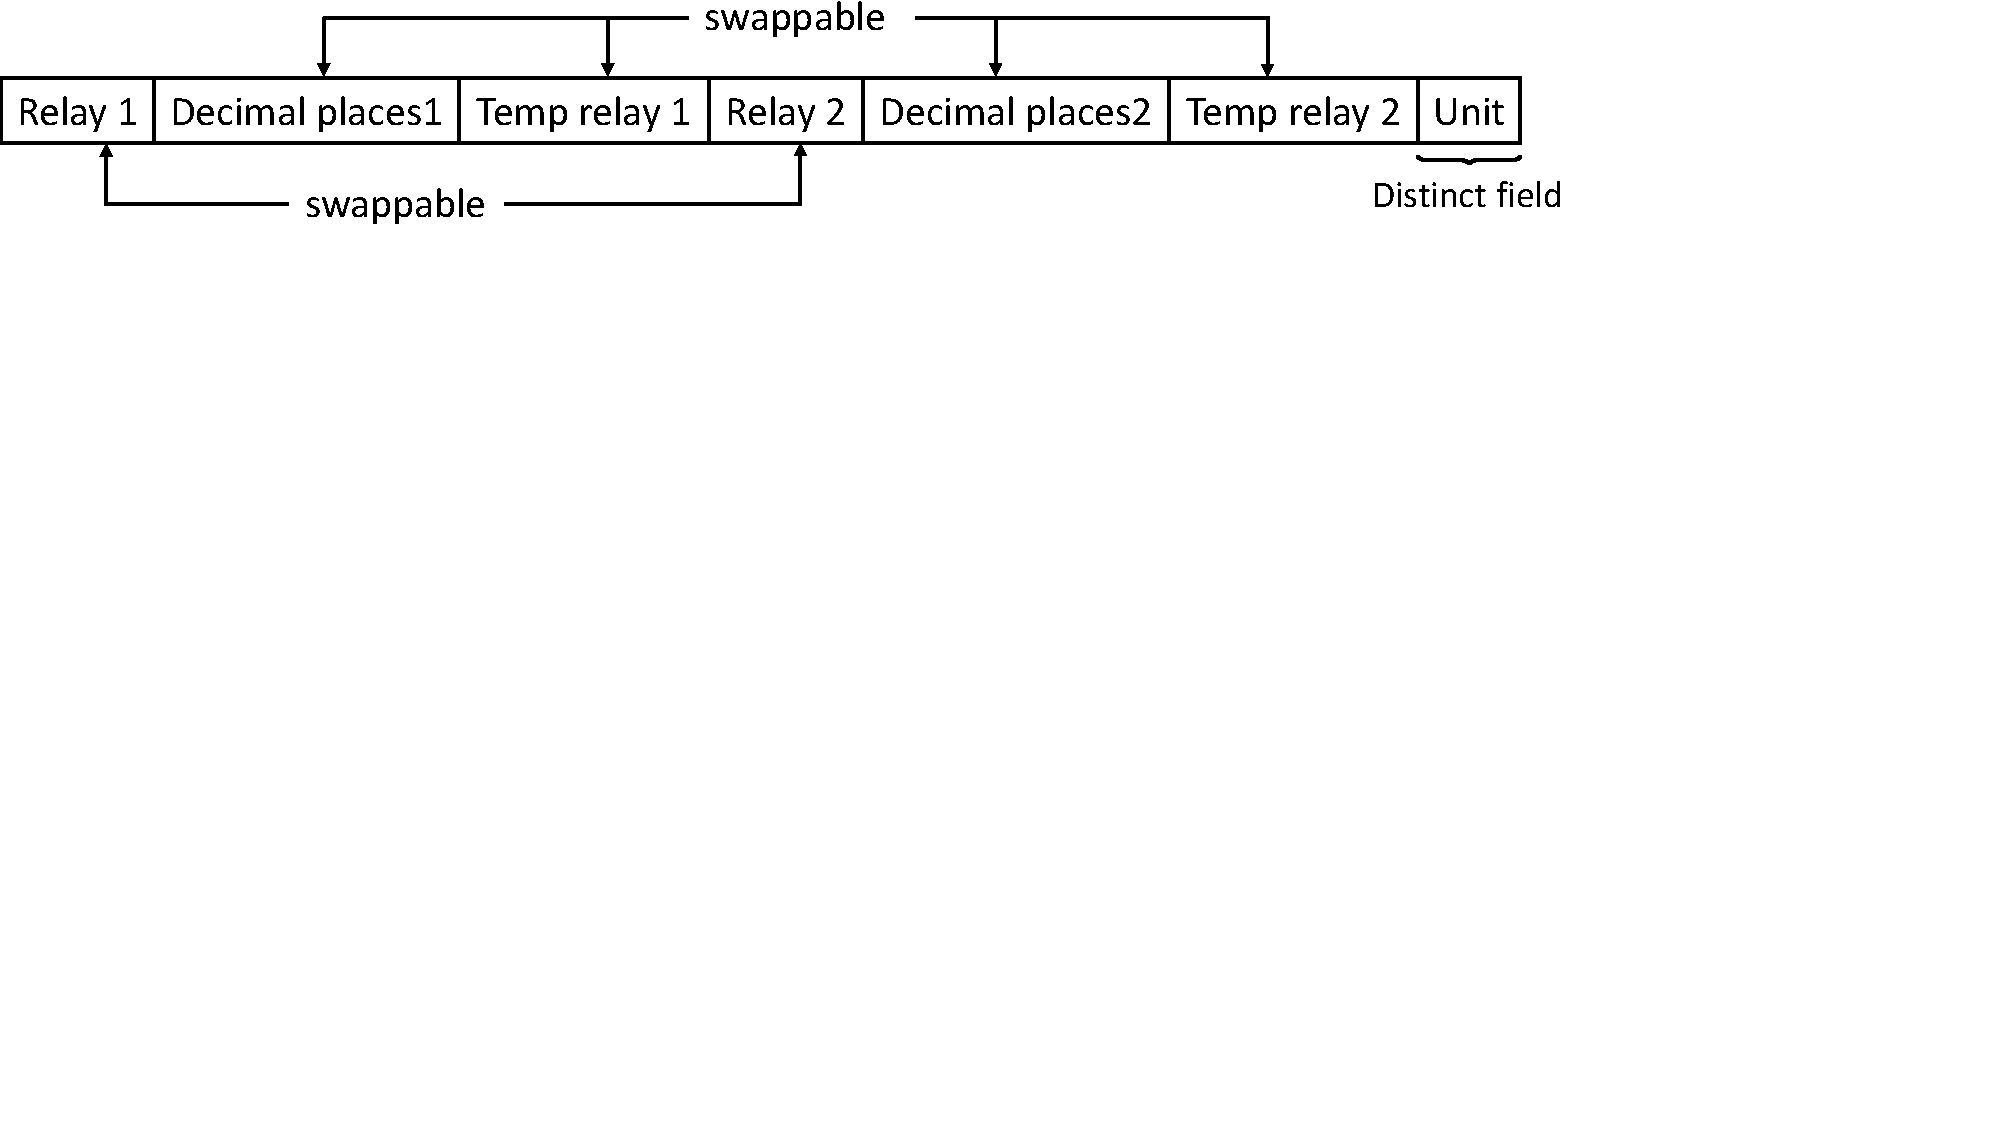
\includegraphics[trim={0 15cm 7cm 0},clip,width=\linewidth]{FieldPayload_revised.pdf}
 \caption{An example what the server expects from the browser when the user submits a form. We have used the specification illustrated in the Specification~\ref{snippet:specificationXML}. This figure indicates the group of fields that are swappable.}
 \label{fig:payload}
\end{figure}

\begin{figure}[t]
 \centering
 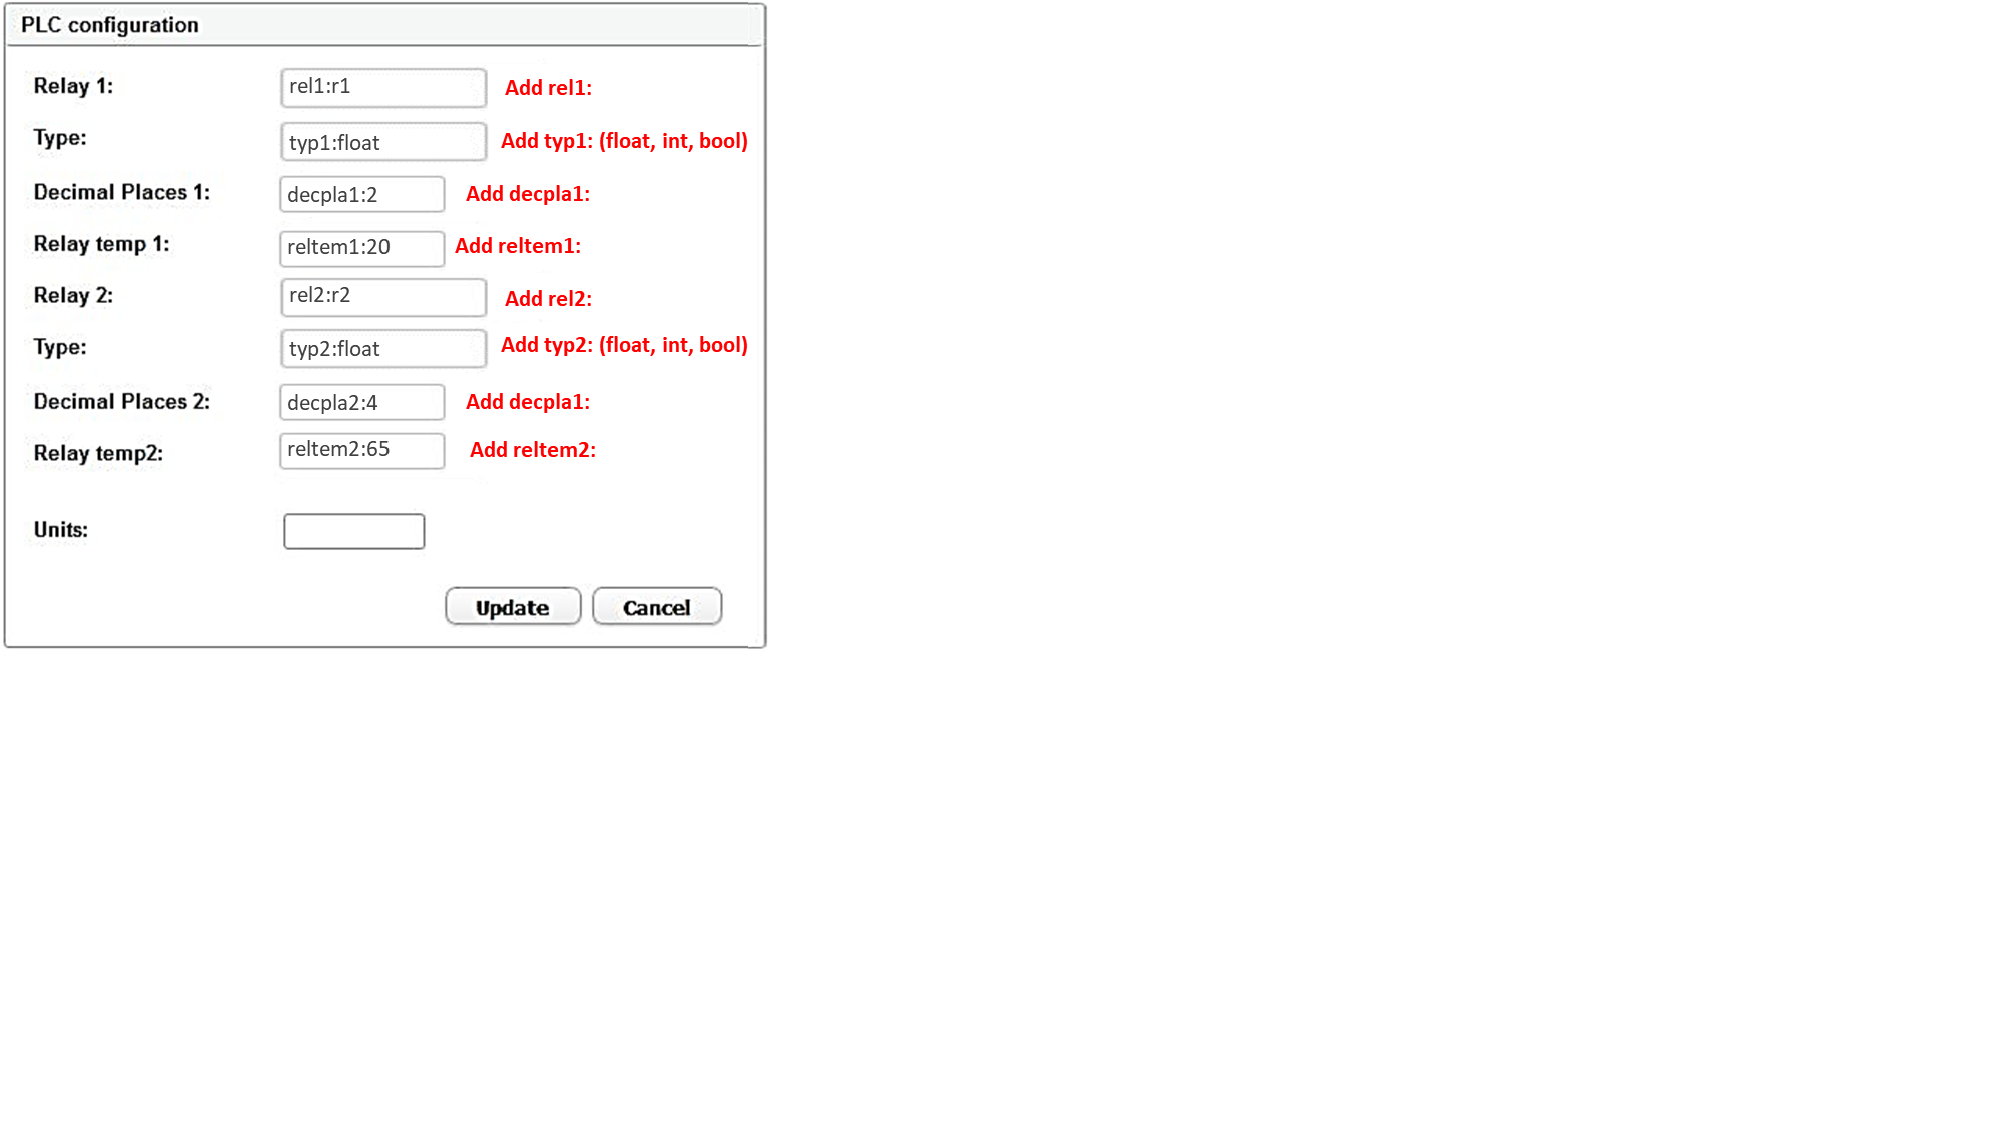
\includegraphics[trim={0 8cm 19cm 0},clip,width=\linewidth]{labelExample_revised.pdf}
 \caption{Example PLC configuration page where the user fill up the text fields with the data and the labels of the text field. E.g., The field \texttt{Relay temp 1} is filled with ``temp1:$20$'' where temp1 is the label to identify the specific text field (\texttt{Relay temp 1}) and $20$ is the actual data.} 
 \label{fig:labelEx}
\end{figure}

\begin{mylist}
  \item First the server checks the number of field data corresponding to the webpage. If it matches with the number of input from the \device, the server proceeds to the next step. There may exist some optional fields that are not required to be filled by the user.
   \item After that, the server matches the data from the browser (\https) and the \device (\tls) and executes the signature verification. If they match, the server proceeds to the next step. Otherwise, it rejects the data and sends a feedback to the \device.
  \item Upon successful matching of the data received from the browser and the \device, the server searches for the input field labels that are added to the data. When found, the server splits the data from the label and parses it. After parsing, the server checks if the data satisfies the specification that is provided to the \tool tool (by matching the data with the regular expression and value/length constraint in the specification). In case the server does not find the label with the data for the overlapping fields, it rejects the data.
\end{mylist}


\subsection{User Side Mechanisms}
\label{sec:fieldSwap:userSide} 

The \device, which is connected to the host system at the user's side, executes the following steps:
\begin{mylist}
  \item As described in the previous section, the browser creates a \https ($TLS_1$) connection to the remote server. \device creates another \tls channel ($TLS_2$) with the remote server by leveraging \webusb API.
 
  \item The server sends the web page containing the input fields to the browser. The server also embeds a text message specifying the input fields that require the user to add the field label. The user fills up the forms.
  
  \item When the user submits the form, the browser sends the form data through the \https ($TLS_1$) connection and the \device sends the data via the $TLS_2$.
\end{mylist}

\iffalse
\subsection{Security Analysis}
\label{sec:fieldSwap:securityAnalysis}

\myparagraph{Attacker model}
As before, we assume a strong attacker that compromises the host system and the network. As the host system is compromised, the attacker can intercept and manipulate any user input and change any visual elements displayed to the user. In Section~\ref{sec:systemDesign}, we address the basic attack where the attacker only changes the input data provided by the user through the input peripherals. In this section, we concentrate on the attack where the attacker swaps the labels of the input fields arbitrarily in a single web page or across a set of web pages.

\myparagraph{Analysis}
We introduce the \tool tool in Section~\ref{sec:fieldSwap:serverSide} to analyze the web pages and calculate the overlapping input fields from the developer given specification. After the analysis, the server includes a text message on the web page instructing the user to add the label to the input filed with the input data. 

The fields that are not overlapping with any other input field do not require the user to add the label. If the attacker executes the swapping attack on such fields, the server can easily recognize such data (due to their distinct specification) and reject them. For the rest of the overlapping fields, the user provides a (label, data) pairing of the input data. Note that the \device sends the signed (label, data) pair using the dedicated \tls channel. This ensures that any manipulation attempt by the malicious host would readily be detected by the server. Swapping across the set of web pages can be prevented if the developer provides the combined specifications sampled from a number of web pages together.

\fi





